% !TEX encoding = UTF-8 Unicode
\documentclass[11pt]{article}
\usepackage{geometry}                % See geometry.pdf to learn the layout options. There are lots.
\geometry{a4paper}                   % ... or a4paper or a5paper or ...
%\geometry{landscape}                % Activate for for rotated page geometry
%\usepackage[parfill]{parskip}    % Activate to begin paragraphs with an empty line rather than an indent
\usepackage{graphicx}
\usepackage{amssymb}
\usepackage{epstopdf}
\usepackage[T1]{fontenc}
\usepackage[utf8]{inputenc}
\usepackage{hyperref}

\usepackage{helvet}
\renewcommand{\familydefault}{\sfdefault}

\renewcommand{\labelitemi}{$-$}

\DeclareGraphicsRule{.tif}{png}{.png}{`convert #1 `dirname #1`/`basename #1 .tif`.png}

% here insert the full path to your BibTeX file
\newcommand{\myreferences}{/Users/matteo/Documents/My\ Library.bib}

\title{The analysis of eye movements as a tool for investigating cognitive processes}
\author{
        Matteo Lisi \footnote{\scriptsize{This chapter was written while the author was working at the Laboratoire Psychologie de la Perception, Université Paris V Descartes. This version has been translated in english from the original italian version published in \href{https://www.mulino.it/isbn/9788815272119}{\textit{Il cervello al lavoro. Nuove prospettive in neuropsicologia}, editors Patrizia Bisiacchi and Antonino Vallesi (2017, il Mulino, ISBN 978-88-15-27211-9)}. The chapter has been translated with the help of an AI tool: from a quick read the translation seems OK, but if you find sections that lacks clarity or could be improved please do let me know. Released under a \href{https://creativecommons.org/licenses/by/2.0/}{CC BY license}.}} \\
        \small{Department of Psychology}\\
        \small{Royal Holloway, University of London}
}
\date{}

\begin{document}
\sloppy
\maketitle

\begin{abstract}
The study of eye movements is an important source of information for both clinical and experimental psychology and neuropsychology. In the first part of this chapter, the different types of eye movements and their functions will be described. In the second part of the chapter, the relationship between eye movements and visual perception will be discussed, and a number of case studies will be presented in which the analysis of eye movements has provided important information regarding cognitive processes such as attention and numerical cognition. Although the chapter will be mostly devoted to the rotational movements of the eye in the orbit, the dilation and constriction movements of the pupil will also be briefly discussed. The chapter will conclude with a brief description of the techniques and methodologies used to record eye movements.
\end{abstract}

\section{Taxonomy and function of eye movements}
Eye movements lie at the intersection of the motor and perceptual functions of the brain. On the one hand, it is a motor action: the act of moving the eyes begins with the activation of a population of neurons, and ends with a contraction or relaxation of the eye muscles in the orbit. Eye movements, however, perform a very specific function: to enable visual perception, i.e. the processing of information from the outside world through the sense of vision.

Vision begins when light enters the eye and reaches the retina, modulating the activity of photoreceptors. Visual acuity—which can be roughly defined as the clarity of vision, or the ability to resolve and perceive fine details—is not uniform across the visual field. It is highest in the central region, at the \textit{fovea}, where the density of photoreceptors is greatest, and decreases exponentially with distance from the centre (cf. fig.\ref{fig1}). Even within the fovea, visual acuity is not uniform and peaks in a very limited region (called the \textit{foveola}), about 0.3 mm in diameter, which corresponds to about 1 degree of visual angle\footnote{Degrees of visual angle ($^{\circ}$) are the units in which both the rotations of the eye and the size and position of objects in the visual field are measured. For example, if a visual stimulus is positioned 10$^{\circ}$ away in a certain direction from the centre of the visual field, in order to centre it on the fovea the eye must make a 10$^{\circ}$ rotation in the orbit in the same direction. The visual angle $\alpha$ (in degrees) subtended by an object of length $l$ positioned at distance $d$ from the eye can be calculated using the following formula $\alpha = 2 \arctan(\frac{l}{2d}) \frac{180}{\pi}$. Approximately, an object 1 cm long and positioned 57 cm from the eye subtends 1$^{\circ}$.}. Despite its small size, the fovea is of enormous importance in the processing of visual information: it is estimated that around 50\% of the visual cortex is dedicated to processing information from the fovea, despite the fact that the fovea represents only 1\% of the retina.

\begin{figure}
\centering
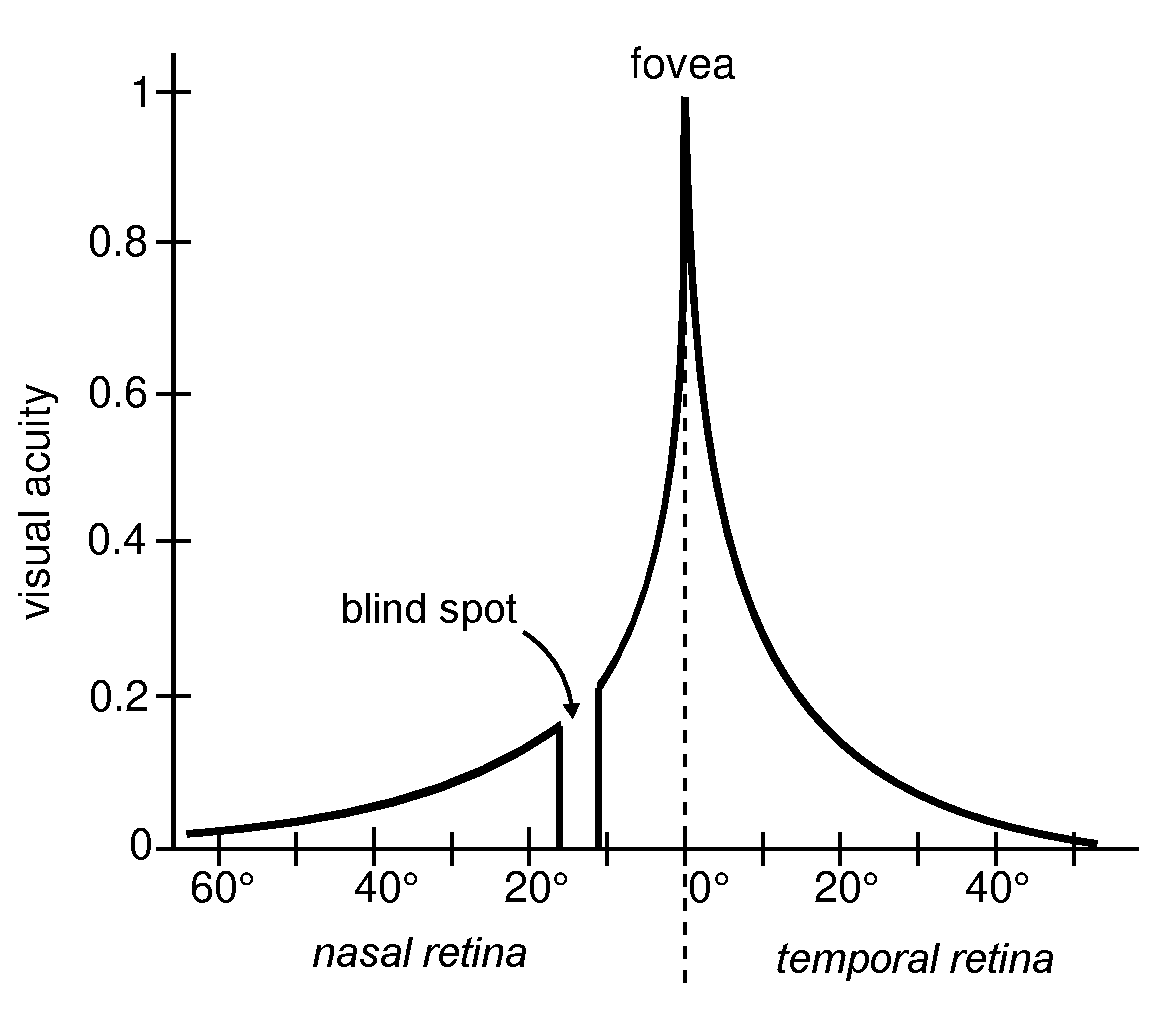
\includegraphics[width=80mm]{fig1.pdf}
\caption{The graph shows how visual acuity decreases rapidly as one moves away from the fovea, represented as a function of retinal distance. The \textit{blind spot}, indicated in the figure, is the point where nerve fibers from various parts of the retina converge to form the optic nerve; since the blind spot contains no photoreceptors, this part of the retina provides no visual information.}

\label{fig1}
\end{figure}

From a functional point of view, therefore, eye movements allow the gaze (or more precisely the visual axis, i.e. the imaginary line that connects an observed object to the centre of the fovea) to be oriented in such a way that the projection on the retina of the object of interest is located close to the fovea (where visual acuity is at its maximum). This strategy (orienting the fovea towards objects of interest) is an evolutionary solution that allows our visual system to quickly analyse the salient elements of our surroundings in detail. The advantage of this solution is parsimony: if we had the same level of visual acuity in the fovea throughout the visual field, the amount of incoming visual information would be such that we would need a visual cortex tens (if not hundreds) of times larger to process it. Another important function of eye movements is to stabilise the gaze in case the observed object, or the observer (or both) are in motion: in fact, to maintain an acceptable quality of vision it is necessary that the speed of retinal slip (the motion of the visual image projected on the surface of the retina) is less than 2-3$^{\circ}$/sec (degrees of visual angle per second).

These two functional goals of eye movements (orienting and stabilising gaze) are achieved through two major classes of distinct movements: rapid movements, also known as saccadic movements or saccades, and slow movements \cite{Steinman1990}. Saccades are extremely rapid movements that move the gaze from one point to another in the visual field. For example, saccades are the movements with which you moved your gaze from one word to another while reading this text. An example of a slow movement, on the other hand, is provided by tracking movements, which are used to keep the fovea oriented towards a moving object, such as a running player or a ball that has just been kicked during a ball game. Slow movements are characterised by a much more variable speed profile than saccades, which is largely dependent on the characteristics of the visual stimulation: for the execution of a pursuit movement, something must be moving in the visual field, and the speed of gaze movement reflects the speed of the stimulus.

Eye movements are also divided into conjugate eye movements, in which the two eyes move in the same direction, and disconjugate (or disjunctive) eye movements, in which the two eyes move in different directions. An example of disconjugate movements are vergence movements, which consist of converging or diverging the eyes so as to ensure that when we move our gaze from a distant object to a near one (or vice versa) the projections of the object of interest lie on the fovea in both the retinas of our left and right eye. The vergence movements are accompanied by the process of accommodation, i.e. the adjustment of the curvature of the crystalline lens, the transparent organ located inside the eyeball that together with the cornea acts as a lens, allowing light rays to be focused on the retina.

Eye movements can then be further subdivided into multiple subsystems, and multiple eye movement classification schemes have been proposed in the literature. Table \ref{tab1} summarises one of the most commonly used classifications, due to Robinson \cite{Robinson1968}, which distinguishes five main types of eye movements. It is important to emphasise that each classification depends mainly on the criteria adopted and that it is difficult to make 'rigid' classifications: normally, the different functions of the eye are performed through the cooperation of different types of eye movements. For a more detailed description of the various types of eye movements, including those of the reflex type, we refer the reader to specialised texts such as Leigh and Zee's excellent handbook \cite{Leigh2015}. In this chapter we will restrict ourselves to a few voluntary eye movements, saccades and slow pursuit movements, which are perhaps most interesting for the investigation of cognitive processes.

\begin{table}
\centering
\caption{Classifications of eye movements.} \label{tab1}
\begin{tabular}{p{5.3cm}p{8cm}}
  \hline
\textbf{Movement type}  & \textbf{Funzione}\\
  \hline  \hline
Vestibulo-ocular reflex & Stabilising retinal image during head movements \\  \hline
 Optokinetic reflex & Stabilising the retinal image during retinal slip of the visual field (e.g. when from inside a moving train we watch the landscape slide out of the window)  \\  \hline
  Saccades & Shifting gaze so as to centre objects of interest on the fovea  \\  \hline
  Slow pursuit & Move the eyes to follow a moving object so as to keep it centred on the fovea  \\  \hline
 Vergence & Moving the eyes in opposite directions so that the projections of an object are centred on the fovea of both eyes simultaneously \\  \hline
   \hline
\end{tabular}
\end{table}

\subsection{An overview of the physiology of the oculomotor system}
Eye movements are determined by the action of 6 muscles (the so-called extrinsic muscles of the eye), organised in 3 pairs with antagonistic action. They are made up of striated fibres, originate from the optic canal, at the bottom of the orbit (where the optic nerve also passes through), and end by inserting on the sclera (the outer layer of the eyeball). The coordinated activation of these muscles allows the eyeball to move in the orbit with 6 degrees of freedom. Three of these are translations, which have a minimal amplitude and will be neglected in this chapter. The other 3 are rotations that allow the eye to rotate around 3 different axes, and are achieved by the contraction of one muscle and the relaxation of its antagonist. The combined activation of the 3 pairs of muscles can thus make the eyeball rotate around 3 axes: a vertical axis, a horizontal axis, and the visual axis (so-called torsion movements). Rotations around the vertical axis allow horizontal eye movements, called abductions when they are in the temporal direction and adductions when they are in the nasal direction, and are obtained by contraction/relaxation of the medial and lateral rectus muscles. Rotations around the horizontal axis, on the other hand, result in vertical eye movements called elevation and depression. Vertical eye movements, along with torsional movements, are mainly obtained through the involvement of the superior and inferior rectus and superior and inferior oblique muscles.

The ocular muscles are innervated by the III, IV and VI cranial nerves from the oculomotor nuclei of the brainstem. In particular, the III cranial nerve innervates the superior rectus, medial rectus, inferior rectus, and inferior oblique muscles; the IV cranial nerve innervates the superior oblique muscle, while the VI cranial nerve innervates the lateral rectus muscle.

\subsection{Saccadic eye movements}
Saccades are rapid, conjugate movements of the eyes that are used to orient the foveae to a new position in the visual scene. The study of saccades dates back to at least the end of the 19th century, when the French ophthalmologist Louis Émile Javal (1839-1907) observed that during reading, the gaze is not moved along the line of text in a fluid and continuous manner, but through a series of discrete, very fast movements (in French, the term 'saccade' indicates precisely a sudden and rapid movement), interspersed with pauses in which the gaze remains stationary (fixations).

Saccades can be controlled voluntarily: we can always decide when and where to move our gaze. However, in everyday life they are mostly generated unconsciously and automatically: even if we do not pay attention to them, our eyes are never still, and on average we make 3 saccades per second. Saccades can also be generated reflexively/involuntarily, in response to a sudden stimulus, such as when something appears in the periphery of our visual field attracting our attention and gaze. Saccades are not limited to visual stimuli: for example, it has been shown that in complete darkness tactile stimulation of a hand typically results in a saccadic movement directed towards the stimulated hand \cite{Groh1996}. The latency of a saccadic movement in response to a displacement of the observed object or the appearance of a new peripheral stimulus is around 200-250 milliseconds, and is influenced by numerous factors such as brightness, target distance, and presence of distractors.

As we have mentioned, saccades are also called rapid movements: they are in fact one of the fastest movements produced by the human body. During a saccade, the speed of rotation of the eye in the orbit can reach peaks of around 900$^{\circ}$/sec. Given the extreme speed of saccades, it is natural that it is very difficult to change their trajectory 'on the fly'. In fact, saccades are considered a ballistic type of movement: once started, its amplitude and direction cannot be changed. Moreover, they are characterised by a stereotyped acceleration/deceleration profile over which we have no voluntary control: they begin with a rapid acceleration, culminating in the first half of the saccade, followed by a rapid deceleration. There is a relatively stable relationship between amplitude and velocity (and consequently also duration) of a saccade: peak velocity increases almost linearly with amplitude (see figure \ref{fig2}), up to amplitudes around 20$^{\circ}$, which tends to saturate and flatten out progressively for amplitudes above 20$^{\circ}$. This regularity is referred to in the literature as the main sequence, a term borrowed from astronomy (where it indicates the relationship between the brightness and temperature of a star), and has been used in eye movement research to determine whether or not a certain type of observed movement can be considered a saccade (i.e. has been generated by the same control system that generates saccades) and in the clinical field to characterise abnormalities of saccadic movements. The duration of a saccade therefore depends on its amplitude, but is generally very short: typically around 50-100 milliseconds for saccades of amplitude around 5-10$^{\circ}$, but saccades of greater amplitude can be up to 200 milliseconds.

Saccadic movements reorient the visual axis towards elements of interest. It is therefore interesting to ask how accurately they manage to hit their targets. We should note that not all saccadic movements are directed towards a well-defined, small target (a point target): very often saccades are performed with the simple purpose of repositioning the visual field, without necessarily being directed towards a particular element of the visual scene.

In particular, saccades to targets at distances greater than approximately 5$^{\circ}$ tend to be hypometric, i.e. their amplitude on average tends to cover only 90\% of the target's distance. Several theories have been proposed to explain this phenomenon: for example, since the duration of a saccadic movement tends to increase with its amplitude, it has been suggested that saccades are programmed to minimise execution time \cite{Harris1995}. However, it should be remembered that when a saccade terminates far from its target, it is typically followed by a secondary saccade characterised by small amplitude and very short latency (often less than 100 milliseconds) that corrects the error of the initial saccade \cite{Jacobs1987}. Furthermore, under more ecological conditions, i.e. where the targets are stable (instead of suddenly appearing and disappearing as is the case in many experimental protocols) and the timing of the eye movement is freely decided by the subject, the saccades tend to be more accurate and show only a small constant error that does not increase as a function of the amplitude of the saccade \cite{Collewijn1988}. Finally, under ecological conditions each saccadic movement is typically accompanied by a head movement that tends to compensate for the hypometry and increase the accuracy \cite{Guitton1987}.\footnote{\scriptsize{See Lisi et al 2019 for a more recent perspective on saccade hypometria \cite{Lisi2019}.}}


\begin{figure}
\centering
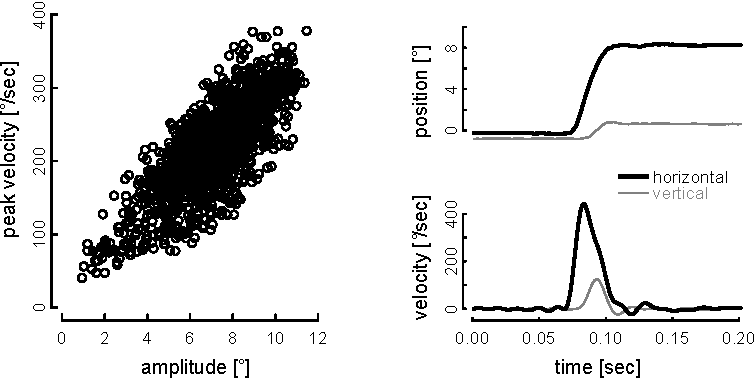
\includegraphics[width=140mm]{fig2.pdf}
\caption{The graph on the left shows the typical main sequence of saccades: a linear relationship between amplitude and peak saccade velocity. Each point represents a saccadic movement made by a subject during the course of an experiment. On the right is the oculographic trace of a single saccadic movement: the top panel shows the position of the gaze (calculated in degrees of visual angle relative to the centre of a computer screen) as a function of time; note the typical step shape, indicating a rapid movement of the gaze from one side of the screen to the other. Below is the speed of gaze movement: note the typical rapid acceleration/deceleration profile that characterises rapid eye movements}.
\label{fig2}
\end{figure}


How does the accuracy of eye movements change as we age? The somewhat surprising answer is that accuracy remains fairly constant \cite{Warabi1984}, while other parameters, such as duration and latency, change significantly \cite{Munoz1998}. With increasing age there are physiological changes, e.g. in the rigidity of the eye muscles, that make eye movements more difficult. Despite this, our oculomotor system is able to learn, or rather adapt the impulses it sends to the oculomotor neurons to counteract these variations, allowing a constant level of accuracy to be maintained. These adaptive processes can also be demonstrated in the laboratory: if we ask a subject to perform a saccade to move their gaze to a peripheral target, but each time during the execution of the movement we move the target slightly (e.g. by increasing the distance by 15\%), the oculomotor system will adapt in a short time, and will begin to respond with increasingly larger saccades, a phenomenon called saccadic adaptation\cite{McLaughlin1967}. Saccadic adaptation is a form of sensorimotor plasticity that, given the ease with which it can be elicited, is often used as an experimental model for studying sensorimotor learning.

\subsection{Fixations}
Fixations are the pause periods - between one eye movement and the next - during which our visual perception occurs. Fixations have a highly variable duration that depends on a multitude of factors, related both to the characteristics of the observed image and to the observer's objectives and mental states. During the exploration of a visual scene, we move from minimum durations of around 100 milliseconds to much longer fixations that can last even more than 2-3 seconds. It is important to emphasise that, from the point of view of motor control, fixations do not consist in the simple absence of an oculomotor command; instead, they are the result of a sophisticated mechanism aimed at stabilising the gaze on the target, so as to maintain its image on the fovea and allow it to be analysed by the visual system. Gaze stabilisation is also ensured by the collaboration of the slow tracking system, and the vestibulo-ocular and optokinetic reflexes (see Table \ref{tab1}).
Although the eyes appear stationary during fixations, in reality they are never perfectly still but continue to move imperceptibly. These microscopic movements made during fixations are subdivided into:
\begin{itemize}
\item \textit{microsaccades}, that is saccadic movements of very small amplitude, around 0.1$^{\circ}$;
\item \textit{ocular drift},  slow, meandering movements occurring between one microsaccade and another;
\item \textit{tremor},  a rapid, tiny oscillation that occurs jointly with the ocular drift.
\end{itemize}
These microscopic eye movements have multiple functions. First of all, they shift the visual image on the retina, causing continuous variations in the incoming visual signals and making it possible to avoid neural adaptation phenomena that could cause the progressive evanescence of static parts of the visual scene (a phenomenon known as the Troxler effect, first described by the Swiss philosopher Ignaz Paul Vital Troxler in the early 1800s).

In addition, more recent studies have shown that these microscopic movements, always present during ocular fixations, reformat the incoming visual information in such a way as to equalise the spectrum of spatial frequencies that make up the image, emphasising the higher spatial frequencies \cite{Rucci2015} and thus improving sensitivity to fine image details. Finally, it has been shown that microsaccades can also be used to position objects of interest at the foveola during tasks that require the perception of particularly fine details, on the order of a few hundredths of a degree of visual angle \cite{Ko2010a,Rucci2007}.

\subsection{Slow pursuit movements}
Slow pursuit movements aim to maintain images of moving objects on the fovee. From a motor point of view, they are very similar to the optokinetic reflex; however, whereas the optokinetic reflex is reflexively generated in response to retinal gliding of the entire visual field, the pursuit movement is voluntarily generated in order to keep an object moving on the fovea independently of its context. The execution of a slow pursuit movement is characterised by a latency (the interval from the onset of target movement to the onset of eye movement) of approximately 100 milliseconds.

Despite their connotation as 'slow' movements, these eye movements can reach quite high speeds, up to about 100 $^{\circ}$/sec. The efficiency of this movement is quantified by calculating its gain, i.e. the ratio of the speed of gaze movement to the speed of the target. A gain value of 1 would therefore indicate that the eyes are moving at the same speed as the target; however, the gain of slow pursuit movements is typically less than 1, particularly for very high target speeds. Since the gain tends to be less than 1, in order to prevent the gaze from falling behind the target, saccades of small amplitude are often performed, which serve to reduce and maintain the gap between target and visual axis at acceptable levels.

Despite being initiated voluntarily, the slow pursuit movement is entirely determined by the visual stimulus. It is in fact impossible to move the eyes in a slow, fluid motion without a moving target to follow. If you try to move your eyes slowly between two fixed points in space, e.g. the left and right margins of this page, the only thing you will be able to produce is a sequence of small saccades. During the pursuit of a target, on the other hand, the slow movement characteristics reflect the movement of the target: if the target changes speed or direction, the eyes follow it step by step, with a delay of about 100 milliseconds. In addition, slow pursuit movements also have a predictive component, which cannot be explained in terms of reflex behaviour. This predictive component is evident in experiments in which subjects are asked to follow with their gaze moving stimuli that change direction in a periodic and predictable manner (e.g. a target moving back and forth on a horizontal path): in these cases it was observed that the gaze movement is able not only to follow changes in the direction of the stimulus without delay, but also to anticipate them. Furthermore, if after a few seconds of ocular pursuit the target is suddenly made to disappear, the slow pursuit movement persists, albeit quickly, continuing along the same trajectory \cite{Whittaker1982}. Since there is no longer any incoming visual information after the disappearance of the target, the speed and direction of the eye movement can only be guided by an 'internal model', i.e. a representation of the characteristics of the target's movement that allows its subsequent movements to be anticipated. The control of slow pursuit movements is therefore not solely determined by visual stimulation, but also depends on an internal model, the nature of which is still debated, but which probably reflects not only the physical characteristics of the stimulus but also more typically cognitive factors such as memory and attention.

\subsection{Eye movements and visual perception}
Our visual perception is an active process: the world we see is not simply a passive reading of incoming sensory information, an impression dictated directly by the light profile hitting the retina. Instead, our visual perception is an active construction based on the combination of incoming sensory information with other information of \textit{extra-retinal} origin, i.e. not visual but motor. This concept can be more easily understood through an example. We have mentioned that on average we produce a saccade every 3 seconds, and each of these shifts of the visual axis causes drastic changes in the image projected onto the retina. In the absence of additional information, these changes could be interpreted - in principle - either as a reorientation of the retina, caused by a movement of the eyes, or as a movement of the entire surroundings that occurred while the eyes and the observer remained still. Despite this, our perception is that of a 'stable' world: we do not perceive the world moving when we move our eyes. This problem is known in the literature as the visual stability (or spatial constancy) problem, and indicates that our perception is not only dependent on visual signals from the retina, but also on motor signals that encode eye movement.

What happens when the image on the retina moves in the absence of a simultaneous motor signal? While keeping one eye closed, try tapping the outer edge of the open eye with your finger so that it moves slightly. You will get a vivid impression of movement of the visual scene. This simple observation (already carried out by Purkinje in the last century \cite{Purkinje1825}) shows that the information coming from the retina alone is not sufficient to guarantee spatial constancy, and suggests that our visual system, alerted by the motor signal, 'cancels' the perception of retinal slip of the visual scene that would accompany each eye movement.

During a sequence of saccadic movements, the images projected onto the retina during periods of fixation follow one another in jumps, in an almost discrete manner; despite this, our visual perception is continuous, without apparent interruptions or discontinuities. It has been shown that during each saccadic movement our visual perception is strongly inhibited, a phenomenon known as \textit{saccadic suppression}. \cite{Volkmann1978}. This phenomenon can be demonstrated with another observation: try to stand in front of a mirror and try to see your eye movements, e.g. by moving your gaze from your left eye to your right eye. No matter how hard you try, you will not be able to catch the eye in motion: your eyes will always appear motionless. It is not the case that these movements are too fast for our visual system to perceive: if you stand in front of another person, and ask them to move their gaze alternately from your right eye to your left eye, you will have no problem seeing their eye movements. So what happens to the incoming visual information during the saccade? It seems that this information is simply ignored by the visual system: if you try to make a saccadic movement towards a clock, sometimes the second hand appears to remain stationary in its position for more than a second, a phenomenon called the illusion of a stopped clock or \textit{saccadic chronostasis} \cite{Yarrow2001}. It seems that the brain 'fills' the interval corresponding to the duration of the eye movement with the first image following the saccade, allowing the continuity of our visual perception.

\begin{figure}
\centering
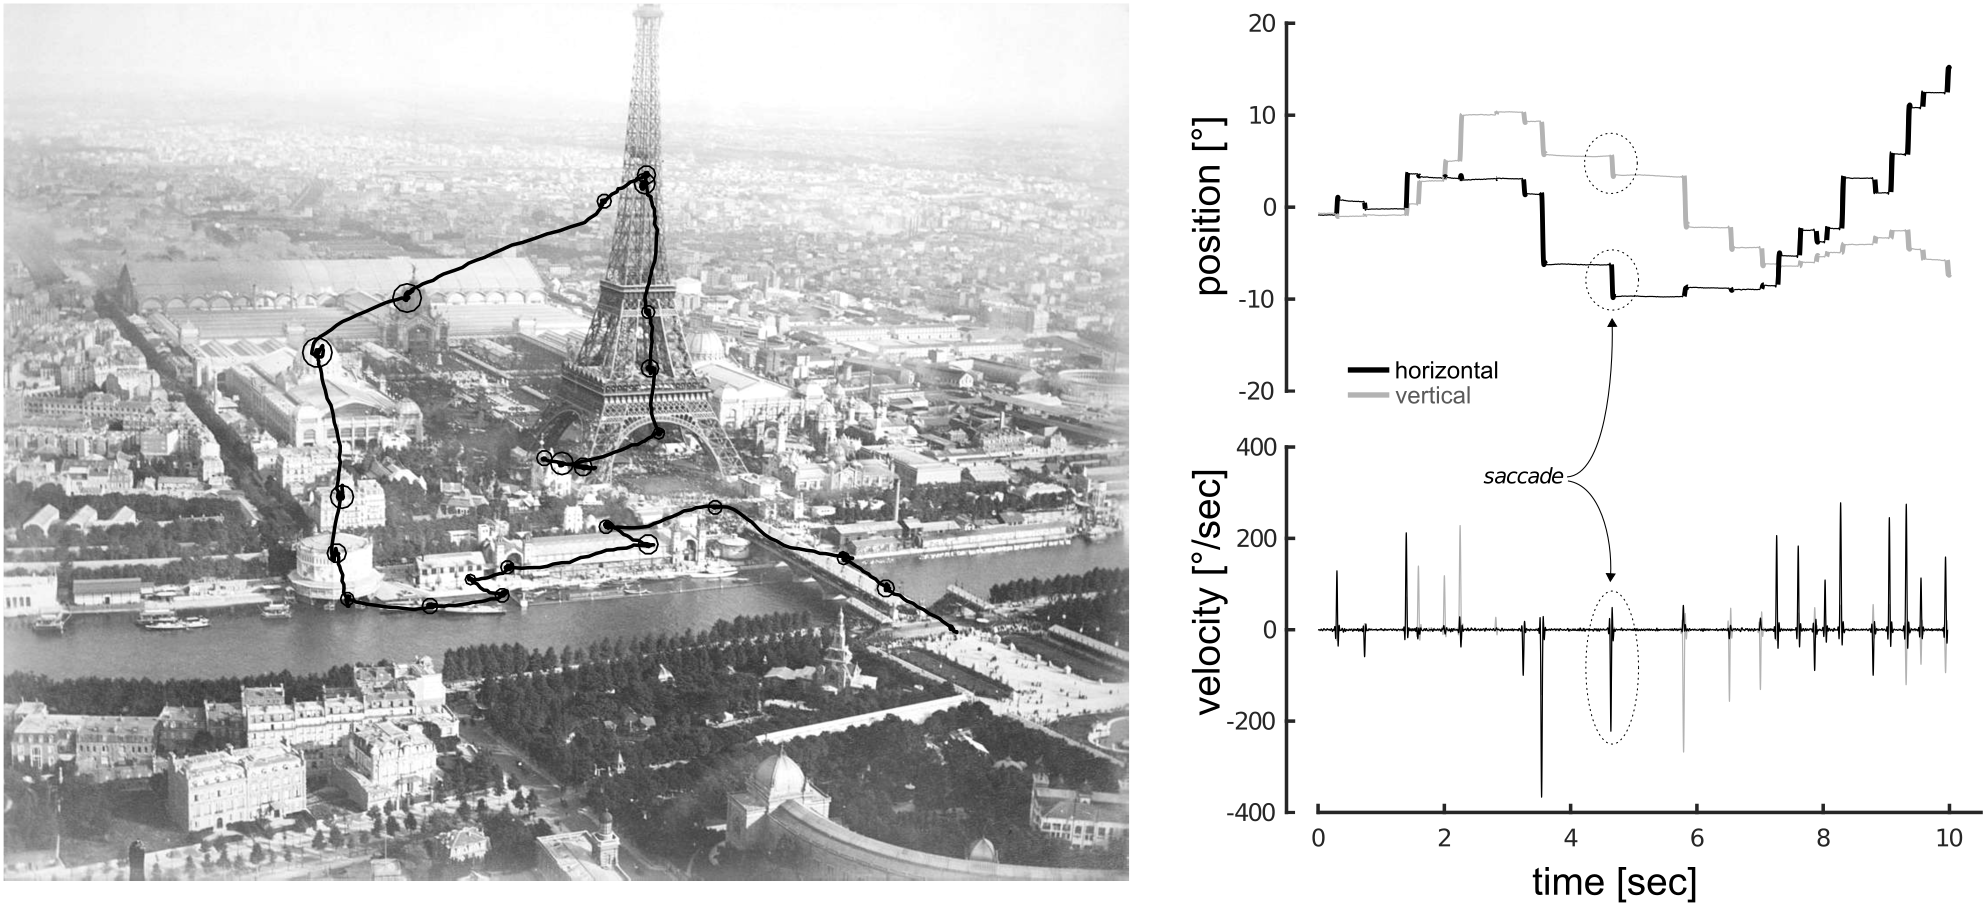
\includegraphics[width=148mm]{fig3.pdf}
\caption{Example of visual exploration of a photograph. The image on the left shows the path taken by the gaze (black line in overlay) of a subject during 10 seconds of free observation of a famous photograph by Alphonse Lièbert (1827-1913), representing an aerial view of Paris during the Universal Exhibition of 1889. Note how the visual exploration follows the prominent elements in the image: it starts in a central position following the Eiffel Tower and then moves on to the main surrounding buildings. In the picture, the circles represent the position of the fixation periods (the diameter of the circles is a function of the duration of the fixation period). The two panels on the right of the photograph represent the oculographic trace of the same 10 seconds of visual exploration: the top panel represents the position (calculated in degrees of visual angle relative to the centre of the photograph) and the bottom panel represents the speed. The oculographic trace illustrates well how visual exploration consists of a series of moments when the eyes are stationary (fixations) and rapid saccadic movements. Analysing the speed of gaze movement makes it easy to identify saccades (which correspond to peaks in speed) and consequently to isolate one fixation from the next. Note how the acceleration and deceleration profile, clearly visible in Figure~\ref{fig2}, here appears almost as a single pulse due to the different time scale}.
\label{fig3}
\end{figure}

\break
\section{Eye movements and cognitive processes}

\subsection{Attention}
Visual exploration behaviour consists of a succession of fixations, interspersed with saccadic movements that orient the fovea towards different parts of the image (an example is shown in figure~\ref{fig3}). The sequence of saccades and fixations performed during the observation of a visual scene is not random but is influenced by the observer's mental states and cognitive goals. One of the first to show this was Alfred L. Yarbus (1914-1986), a Russian psychologist regarded as one of the pioneers in the study of eye movements. Between the 1950s and 1960s, Yarbus used an innovative method for recording eye movements, based on tiny suction cups attached to the surface of the eye, which allowed him to study eye movements with great precision. Yarbus observed that eye movements are not random but are functional to the perceptual and cognitive goals of the observer: when observing a scene, the gaze lingers (both voluntarily and involuntarily) more often and longer on the elements that are likely to provide more information. There is therefore a mechanism capable of filtering information from the peripheral parts of the visual field and selecting the most salient or relevant elements as potential targets for the next saccadic movements. This mechanism is visuo-spatial attention: we look at what attracts our attention.

Numerous studies have shown that there is a close relationship between the preparation of a saccadic eye movement and the orientation \textit{implicit} (i.e. in the absence of a visual axis shift) of spatial attention. For example, it has been observed that the execution of a saccadic movement is necessarily preceded by the orientation of implicit attention towards the target \cite{Deubel1996}. This orientation of attention causes an enhancement in the perception of visual details of the target in the interval immediately preceding the execution of the movement, i.e. before the shift of the visual axis, when the fovea is still oriented towards the initial fixation point. A complementary phenomenon has also been demonstrated: orienting attention to a position in space facilitates the subsequent execution of a saccadic movement towards that same spatial position \cite{Kowler1995}, reducing its latency (which can be defined as the saccadic reaction time, i.e. the interval between the appearance of a target and the execution of a saccade towards it).

Towards the end of the 1980s, Rizzolatti and colleagues were the first to propose that visuospatial attention derives precisely from the activation of the same neural circuits implicated in the programming and execution of saccadic movements \cite{Rizzolatti1987}, formulating the \textit{premotor} theory of attention. According to this theory, implicitly directing attention towards a spatial position is equivalent to programming an eye movement towards that position, but without executing it. This theory was initially proposed on the basis of behavioural experiments, but later also received strong support from neuroimaging studies \cite{Corbetta1998} and neurophysiology studies \cite{Moore2001}.

Interestingly, one of the studies that provided the initial impetus for the premotor theory was based on the analysis of the trajectories of saccadic eye movements. In this study \cite{Sheliga1995}, the trajectories, particularly the curvature, of vertical saccades performed while attention was oriented in the right or left visual hemispace were measured. The intuition behind this study was that if the orientation of attention implies an activation of oculomotor circuits, this activation should manifest itself as a modulation of saccadic movement. The results showed that when attention is oriented towards a visual half-field (right or left), the trajectory of the vertical saccadic movement is not rectilinear but presents a systematic deviation, a curvature in the direction of the opposite half-field (with respect to the focus of attention). The mechanisms by which this modulation of the trajectory of saccadic movements takes place are still debated \cite{VanderStigchel2006}, but it is clear that this result implies a certain degree of overlap between the neural circuits underlying attention and saccadic movements, in agreement with premotor theory and in contrast to previous models of attention, in which attention was seen rather as a supramodal control mechanism anatomically separate from motor circuits. This study is therefore an excellent example of how the analysis of certain parameters of eye movements can provide important elements for understanding more typically cognitive processes such as attention.

\subsection{Numerical Cognition}
In the previous section, the close link between saccadic eye movements and visuospatial attention was briefly illustrated. The orientation of attention in space, however, is not solely involved in guiding eye movements or visual perception. There are in fact other cognitive operations, such as number estimation, or the ability to judge the larger of two numbers, that are thought to require processes very similar to the orientation of attention in space. This hypothesis is supported by a large number of behavioural and neuroimaging studies, which have shown, for instance, how brain areas in the posterior parietal cortex that are implicated in the programming of eye movements also play a role in the mental execution of simple arithmetic operations such as subtraction or addition \cite{Knops2009}. These studies suggest that mental representation is spatial in nature and that the processing of a numerical quantity involves the orientation of spatial attention \cite{Hubbard2005}.

Several researchers in the field of numerical cognition have therefore considered using eye movement analysis to better understand the nature of the mental representation of numbers. Loetscher and colleagues \cite{Loetscher2008} recorded the eye movements of subjects engaged in numerical bisection tasks, consisting of pointing to the number in the middle of a pair of numbers (e.g. the number in the middle for the pair 1-9 is 5). While performing the task, the subjects were in complete darkness, so that they had no incoming visual information that could guide, e.g. automatically or exogenously, their eye movements; the two numbers were presented acoustically. The results showed that the horizontal position of the gaze shifted to the left when the two numbers were presented in descending order (9,1), but not when they were presented in ascending order (1,9). If we consider the shifts of the eyes during the task as the manifestation of shifts of attention in mental number space, these support the hypothesis that mental number space is organised as a mental number line, in which the smallest numbers are represented to the left \cite{Zorzi2002}. In a subsequent study \cite{Loetscher2010}, subjects were asked to produce a random series of numbers, and it was found that the analysis of eye movements (the shifts of the visual axis during the production of the number sequence) made it possible to predict whether the next number in the series would be larger or smaller than the previous one, even before the subject pronounced it. These results thus show how the processing of numerical quantities can modulate the oculomotor system; other more recent studies have taken the opposite approach, and shown how the execution of eye movements, both automatic and voluntary, can influence the concurrent processing of numerical quantities \cite{Ranzini2015,Ranzini2016}. For example, Ranzini and colleagues observed that in a numerical parity judgement task (in which subjects have to indicate as fast as possible whether a number is even or odd), the typical \textit{size effect}, characterised by a slowing of reaction times as the numerical magnitude increases, disappears when subjects simultaneously perform both saccadic and slow pursuit eye movements towards the right side of the visual field. This result supports the hypothesis of a correspondence between visual space and mental numerical space.

In conclusion, these studies, beyond their relevance to theoretical models of numerical cognition, show how the analysis of eye movements can also be useful in the investigation of apparently more abstract cognitive processes, such as those underlying our ability to perform numerical operations.

\subsection{Pupillometry}

In the previous sections we discussed the rotational movements of the eye in the orbit. There is another class of eye movements, which we have not yet mentioned, but which has considerable potential for use in the study of cognitive processes. These are the movements of dilation (also known as \textit{midriasis}) and narrowing (or \textit{myosis}) of the pupil, i.e. the hole located in the centre of the iris that allows light to enter the eyeball and reach the retina. The diameter of the pupil is determined by the contraction of two opposing muscles: the \textit{sphincter pupillae} and \textit{dilator pupillae}. The activation of these muscles is mainly determined by the level of ambient light. The changes in pupil diameter caused by variations in the level of illumination are in fact very large, and easily visible to the naked eye: going from a very brightly lit room to a very dark one can cause a dilation of the pupil diameter up to twice its typical size, which is around 3 millimetres \cite{MacLachlan2002}. Furthermore, since the nerve fibres that mediate pupil dilation and constriction belong to the sympathetic and parasympathetic autonomic nervous systems, respectively, pupil diameter also reflects psycho-physiological states such as the level of arousal. Finally, changes in pupil diameter occur also during accommodation (i.e. the process of adjusting of the shape of the crystalline lens, thus changing the focal length of the eye and allowing it to focus on objects at various distance).

Superimposed on fluctuations in pupil diameter due to arousal, accommodation and reflex to light, there are other variations characterised by a much smaller amplitude (in the order of 0.5 millimetres), which are related to cognitive activity. Since these variations have a very low amplitude, and tend to be masked by the larger variations induced by changes in illumination level or arousal, it is necessary to extract them with a procedure very similar to that used in the analysis of electroencephalographic evoked potentials. In short, the pupillary diameter is recorded for numerous repetitions of the stimulus or task of interest; during the analysis, the different 'epochs' of recording are synchronised with the stimulus events and then averaged so as to isolate the pupillary response caused by the event of interest from the background noise and variations due to other factors (e.g. arousal, or conversely, subject fatigue).

A large number of studies have used this technique (for a review see \cite{Beatty2000}) and shown that a dilation of the pupil diameter accompanies any effort, be it a physical effort (e.g. lifting a weight) or a purely mental effort, such as solving an arithmetic problem \cite{Hess1964} or keeping a sequence of numbers in memory \cite{Kahneman1966}. The mechanisms by which cognitive activity is reflected in the dilation of the pupil diameter are still under investigation, but it is generally believed to be a consequence of the activation of noradrenergic neurons in the locus coeruleus (a brainstem structure) and the consequent release of noradrenaline \cite{Aston-Jones2005}. In particular, pupil dilation would be correlated with an activation of the noradrenergic system, which plays an important role not only in regulating arousal and maintaining the waking state, but also in many other cognitive functions. For example, it is believed to play a role in the control of attention and its focalisation \cite{Corbetta2008}: when attention is focused on a task the noradrenergic system would present a phasic mode of functioning, i.e. characterised by periods of low spontaneous activity interrupted by rapid activations associated with task-related decision-making processes. These phasic oscillations would be reflected in the pupillary diameter and their amplitude would correlate with the attentional load required. In agreement with this hypothesis, it has been shown that, in a task of identifying brief visual and auditory stimuli, the amplitude of the evoked pupillary dilation correlates with the difficulty of the task and with the attentional load required to perform it \cite{Lisi2015b}.

In conclusion, it is worth emphasising that pupillary diameter, due to its relationship with the noradrenergic system, can be useful in the study of many cognitive processes involved in decision-making \cite{Nieuwenhuis2005}, not just attention. It is foreseeable that the measurement of pupil diameter will assume an increasingly important role in the coming years, due in part to the fact that it can be performed very easily and non-invasively.

\section{Eye movement recording techniques}
Early techniques used to analyse or record eye movements were often invasive (e.g. the tiny suction cups applied to the eyes by Yarbus in the 1960s). Other less invasive methods were also less accurate, such as electrooculography (EOG), for example, which is based on the corneo-retinal potential, i.e. the difference in electrical potential, of the order of about 1 mV, existing between the cornea and the \textit{fundus} of the eye (the inner face of the eye, opposite the lens, where the retina is located). Because of this potential, the eye can be regarded as an electrical dipole (with a negative pole on the retina), whose rotations give rise to signals that can be measured by electrodes placed near the eyes. However, the corneo-retinal potential is not constant and is influenced by numerous factors (e.g. illumination and fatigue) through mechanisms that have not yet been fully elucidated; consequently, the accuracy of this technique is very limited.

A much more accurate method of recording eye movements is the scleral coil method (\textit{scleral coil}) which, however, requires the application of a special contact lens, inside of which is the coil. The subject's head in this case must be positioned within a magnetic field: when the coil is immersed in the magnetic field, it generates an electrical potential that is a function of the angle between the orientation of the coil and the direction of the magnetic field. This method offers the best accuracy (in the order of 0.01$^{\circ}$), but because of its invasiveness (the contact lens is particularly uncomfortable due to the presence of the coil and an electrical wire coming out of the lens) it is not used very frequently.

Nowadays, there are instead many oculometry systems called video-based eyetrackers (\textit{video-based eyetrackers}) that, while not being invasive, allow excellent levels of accuracy to be achieved, such that even microscopic eye movements made during fixation periods can be analysed. These systems are based on the analysis of the image of the eye taken by a camera. In order to measure the direction of gaze accurately, the camera is flanked by a light source (typically characterised by a lower frequency than visible light, i.e. in the infrared region). The light from this light source strikes the eye, generating a reflected image, also known as the Purkinje primary image (caused by light reflected off the outer surface of the cornea). In order to distinguish head movements from eye movements, the incoming images from the camera are processed in real time to identify both the Purkinje reflection and the pupil (specifically the centre of the pupil). The position of the centre of the pupil in relation to the Purkinje reflex changes with rotations of the eye in the orbit, but remains relatively constant following small head movements. This method therefore allows eye movements to be isolated from head movements, and accurate monitoring of gaze direction to be achieved even in cases where the head is not perfectly immobilised. Newer models have very high sampling frequencies, up to 2000~Hz, which thus allow eye movements to be recorded with excellent temporal accuracy. The spatial accuracy of these systems can also be further increased if secondary Purkinje images, due to reflections created on the inner surface of the cornea, and on the inner and outer surfaces of the crystalline lens, are included.


\section{Summary}
In this chapter we have described the main types of eye movements, and their functional and physiological characteristics. First and foremost, the study of eye movements plays a fundamental role in the study of visual perception: in fact, we have described vision as an active process, in which the visual experience of the surrounding world depends on the integration of visual information projected onto the retina with extra-retinal signals related to the eye's rotations in the orbit. Furthermore, we have seen how the programming of eye movements is closely linked to the orientation of visual-spatial attention, and how this link allows them to be used in the study of cognitive processes that are apparently more abstract but based on spatially organised mental representations, such as the processing of numerical quantities. Finally, we briefly discussed the dilation and contraction movements of the pupil, and saw how they can provide information on the activity of the noradrenergic system, and thus on all the cognitive processes linked to the neurotransmitter noradrenaline.

In conclusion, we have shown how the analysis of eye movements can provide valuable information regarding a subject's cognitive processes and mental states, and is therefore particularly promising in the field of cognitive neuropsychology, as it can be combined with most currently used experimental protocols with relatively little cost.


\bibliographystyle{abbrv}
\bibliography{\myreferences} % note that this is called using the command defined at the beginning

\end{document}
